\documentclass[10pt]{article}
\usepackage{bytefield}
\usepackage[dvipsnames,table,xcdraw]{xcolor}
\usepackage{adjustbox}
\usepackage{colortbl}
\usepackage{amsmath}
\usepackage{pgf}
\usepackage{tikz}
\usepackage{color,listings}
\usepackage{float}
\usepackage{fancyhdr}
\usepackage{lmodern}
\usepackage[margin=0.5in]{geometry}
\usepackage{setspace}
\usepackage{changepage}
\usepackage{adjustbox}
\usepackage{lastpage}


\pagestyle{fancy}
\fancyhf{}
\lfoot{\thepage}
\rfoot{September 4, 2019}

\def\frontmatter{%
	\pagenumbering{roman}
	\setcounter{page}{1}
	\renewcommand{\thesection}{\Roman{section}}
}%

\def\mainmatter{%
	\pagenumbering{arabic}
	\setcounter{page}{1}
	\setcounter{section}{0}
	\renewcommand{\thesection}{\arabic{section}}
}%

\def\backmatter{%
	\setcounter{section}{0}
	\renewcommand{\thesection}{\Alph{section}}
}%

\begin{document}
\frontmatter
\linespread{1.5}
{\Huge\bfseries  
	\begin{adjustwidth}{100pt}{0pt}
		\begin{flushright}
		\textbf{Universal Serial Bus Communications Class Subclass Specifications for Socket Management Protocol}\\
		~\\
		Revision 0.1\\
		September 4, 2019
	\end{flushright}\end{adjustwidth}\par}
	\clearpage
	{\huge\textbf{Revision History}}\\
	\begin{table}[h!]
		\caption{Revision History}
		\begin{adjustbox}{width=\columnwidth,center}
			\label{tab:revHistory}
			\begin{tabular}{|c|c|p{10cm}|} 
				\rowcolor{lightgray}
				\textbf{Version} &	\textbf{Date} &	\textbf{Comments}\\
				\hline
				1.0 & TBD & Initial Release\\
				\hline
			\end{tabular}
		\end{adjustbox}
	\end{table}
	\clearpage
	
	{\huge\textbf{Contributors}}\\
	\begin{table}[h!]
		\large
		\label{tab:contrib}
		\renewcommand{\arraystretch}{2.0}
		\begin{tabular}{l l} 
			Daniel Berliner & Xaptum\\
			David Bild & Xaptum\\
		\end{tabular}
	\end{table}
	\clearpage
	
	\tableofcontents
	
	\listoffigures
	
	\listoftables
	
	\clearpage
	
	\mainmatter
	\section{Introduction}
	\subsection{Purpose}
	The Socket Control Module (SCM) subclass is a protocol by which USB devices can efficiently manage and use Berkeley/POSIX-style sockets on the host.\\
	\\
	The specification currently defines support for the INET (IPv4) and INET6 (IPv6) protocol families and the TCP and UDP protocols. Future versions may add support for additional families and protocols.\\
	\\
	This protocol offers an alternative method for a device to communicate with remote servers. Existing approaches that operate at the L3 layer (IP/USB) or L2 layer (CDC ECM, EEM, NCM) have several disadvantages.  In particular, they require the device to be assigned an IP address.  Since many networks will assign only a single IP address to a host, this requires implementing some form of network address translation (NAT) on the host.  Setting up the NAT requires userspace configuration in most operating systems, so the USB device is no longer truly plug and play.
	\subsection{Scope}
	This document specifies new device subclasses intended for use with Communication devices,
	based on the Universal Serial Bus Class Definitions for Communication Devices specification
	[USBCDC]. \\
	\\
	The intention of this specification is that all material presented here be upwards-compatible
	extensions of the [USBCDC] specification. New numeric codes are defined for subclass codes,
	protocol codes, management elements, and notification elements. \\
	\\
	In some cases material from [USBCDC] is repeated for clarity. In such cases, [USBCDC] shall be
	treated as the controlling document. \\
	\\
	In this specification, the word ‘shall’ or ‘must’ is used for mandatory requirements, the word
	‘should’ is used to express recommendations and the word ‘may’ is used for options. 
	\section{Overview}
	Socket Control Model (SCM) is a specification for efficent management of sockets on a host by its devices. SCM sends Application Layer traffic and internal socket management commands from the device to the host over USB. This module requires host implementaitons for each suported Network and Transport layer protocols, but other layers are beyond its scope.
	\subsection{What is Socket Control Module (SCM)?}
	SCM allows a USB connected device to remotely create and control sockets on its host. A device may only control sockets it has created, and it shall expect exclusive control over this socket. Devices cannot control sockets created by other devices on the same host, and the host will not expose a devices socket for use by other applications.\\
	\\
	Prior to SCM, connected devices would have to be assigned an IP address requiring the host to bridge the device or use NAT which also requires userspace configurations to the host. SCM allows a host to act on behalf of its device and provice it's network connection in a truly plug and play manner. This implicitly subjects the device to the same firewall rules and external network considerations without specific configuration.\\
	\\
	The below figure illustrates a possible use case where a new socket type (Sock 1) is created on the device to interface with SCM. This allows userspace applications to interact with a standard protocol. 
	\begin{figure}[H]
		\begin{center}
			\caption[SCM Overview]{SCM Overview.}
			\scalebox{0.9}{% Graphic for TeX using PGF
% Title: /home/dev/xaprc00x/rc/EEMDepiction.dia
% Creator: Dia v0.97+git
% CreationDate: Wed Sep  4 16:54:33 2019
% For: dev
% \usepackage{tikz}
% The following commands are not supported in PSTricks at present
% We define them conditionally, so when they are implemented,
% this pgf file will use them.
\ifx\du\undefined
  \newlength{\du}
\fi
\setlength{\du}{15\unitlength}
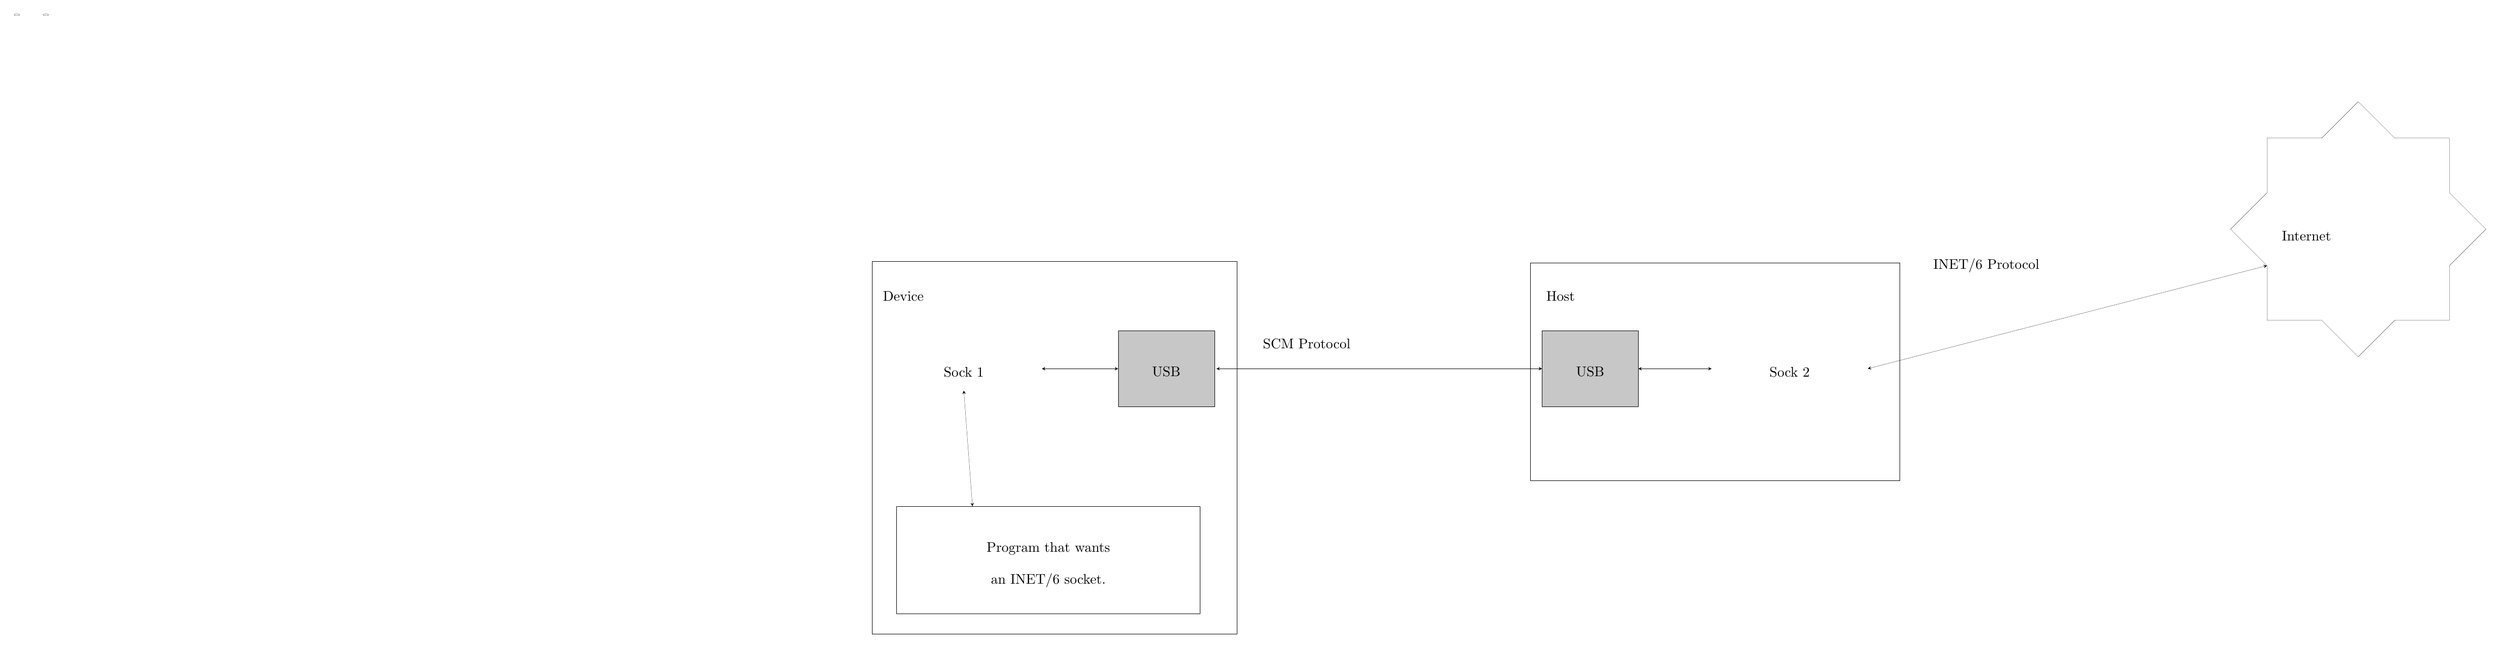
\begin{tikzpicture}[even odd rule]
\pgftransformxscale{1.000000}
\pgftransformyscale{-1.000000}
\definecolor{dialinecolor}{rgb}{0.000000, 0.000000, 0.000000}
\pgfsetstrokecolor{dialinecolor}
\pgfsetstrokeopacity{1.000000}
\definecolor{diafillcolor}{rgb}{1.000000, 1.000000, 1.000000}
\pgfsetfillcolor{diafillcolor}
\pgfsetfillopacity{1.000000}
\pgfsetlinewidth{0.100000\du}
\pgfsetdash{}{0pt}
\pgfsetmiterjoin
{\pgfsetcornersarced{\pgfpoint{0.000000\du}{0.000000\du}}\definecolor{diafillcolor}{rgb}{1.000000, 1.000000, 1.000000}
\pgfsetfillcolor{diafillcolor}
\pgfsetfillopacity{1.000000}
\fill (22.300000\du,6.500000\du)--(22.300000\du,15.850000\du)--(31.450000\du,15.850000\du)--(31.450000\du,6.500000\du)--cycle;
}{\pgfsetcornersarced{\pgfpoint{0.000000\du}{0.000000\du}}\definecolor{dialinecolor}{rgb}{0.000000, 0.000000, 0.000000}
\pgfsetstrokecolor{dialinecolor}
\pgfsetstrokeopacity{1.000000}
\draw (22.300000\du,6.500000\du)--(22.300000\du,15.850000\du)--(31.450000\du,15.850000\du)--(31.450000\du,6.500000\du)--cycle;
}% setfont left to latex
\definecolor{dialinecolor}{rgb}{0.000000, 0.000000, 0.000000}
\pgfsetstrokecolor{dialinecolor}
\pgfsetstrokeopacity{1.000000}
\definecolor{diafillcolor}{rgb}{0.000000, 0.000000, 0.000000}
\pgfsetfillcolor{diafillcolor}
\pgfsetfillopacity{1.000000}
\node[anchor=base,inner sep=0pt, outer sep=0pt,color=dialinecolor] at (26.875000\du,11.370000\du){};
% setfont left to latex
\definecolor{dialinecolor}{rgb}{0.000000, 0.000000, 0.000000}
\pgfsetstrokecolor{dialinecolor}
\pgfsetstrokeopacity{1.000000}
\definecolor{diafillcolor}{rgb}{0.000000, 0.000000, 0.000000}
\pgfsetfillcolor{diafillcolor}
\pgfsetfillopacity{1.000000}
\node[anchor=base west,inner sep=0pt,outer sep=0pt,color=dialinecolor] at (22.575000\du,7.500000\du){Device};
\pgfsetlinewidth{0.100000\du}
\pgfsetdash{}{0pt}
\pgfsetbuttcap
\pgfsetmiterjoin
\pgfsetlinewidth{0.100000\du}
\pgfsetbuttcap
\pgfsetmiterjoin
\pgfsetdash{}{0pt}
\definecolor{diafillcolor}{rgb}{1.000000, 1.000000, 1.000000}
\pgfsetfillcolor{diafillcolor}
\pgfsetfillopacity{1.000000}
\definecolor{dialinecolor}{rgb}{0.000000, 0.000000, 0.000000}
\pgfsetstrokecolor{dialinecolor}
\pgfsetstrokeopacity{1.000000}
\pgfpathmoveto{\pgfpoint{23.294995\du}{8.650000\du}}
\pgfpathlineto{\pgfpoint{25.904995\du}{8.650000\du}}
\pgfpathcurveto{\pgfpoint{26.265361\du}{8.650000\du}}{\pgfpoint{26.557495\du}{8.896243\du}}{\pgfpoint{26.557495\du}{9.200000\du}}
\pgfpathcurveto{\pgfpoint{26.557495\du}{9.503757\du}}{\pgfpoint{26.265361\du}{9.750000\du}}{\pgfpoint{25.904995\du}{9.750000\du}}
\pgfpathlineto{\pgfpoint{23.294995\du}{9.750000\du}}
\pgfpathcurveto{\pgfpoint{22.934629\du}{9.750000\du}}{\pgfpoint{22.642495\du}{9.503757\du}}{\pgfpoint{22.642495\du}{9.200000\du}}
\pgfpathcurveto{\pgfpoint{22.642495\du}{8.896243\du}}{\pgfpoint{22.934629\du}{8.650000\du}}{\pgfpoint{23.294995\du}{8.650000\du}}
\pgfpathclose
\pgfusepath{fill,stroke}
% setfont left to latex
\definecolor{dialinecolor}{rgb}{0.000000, 0.000000, 0.000000}
\pgfsetstrokecolor{dialinecolor}
\pgfsetstrokeopacity{1.000000}
\definecolor{diafillcolor}{rgb}{0.000000, 0.000000, 0.000000}
\pgfsetfillcolor{diafillcolor}
\pgfsetfillopacity{1.000000}
\node[anchor=base,inner sep=0pt, outer sep=0pt,color=dialinecolor] at (24.599995\du,9.400000\du){Sock 1};
\pgfsetlinewidth{0.100000\du}
\pgfsetdash{}{0pt}
\pgfsetmiterjoin
{\pgfsetcornersarced{\pgfpoint{0.000000\du}{0.000000\du}}\definecolor{diafillcolor}{rgb}{1.000000, 1.000000, 1.000000}
\pgfsetfillcolor{diafillcolor}
\pgfsetfillopacity{1.000000}
\fill (38.800000\du,6.550000\du)--(38.800000\du,12.000000\du)--(48.050000\du,12.000000\du)--(48.050000\du,6.550000\du)--cycle;
}{\pgfsetcornersarced{\pgfpoint{0.000000\du}{0.000000\du}}\definecolor{dialinecolor}{rgb}{0.000000, 0.000000, 0.000000}
\pgfsetstrokecolor{dialinecolor}
\pgfsetstrokeopacity{1.000000}
\draw (38.800000\du,6.550000\du)--(38.800000\du,12.000000\du)--(48.050000\du,12.000000\du)--(48.050000\du,6.550000\du)--cycle;
}% setfont left to latex
\definecolor{dialinecolor}{rgb}{0.000000, 0.000000, 0.000000}
\pgfsetstrokecolor{dialinecolor}
\pgfsetstrokeopacity{1.000000}
\definecolor{diafillcolor}{rgb}{0.000000, 0.000000, 0.000000}
\pgfsetfillcolor{diafillcolor}
\pgfsetfillopacity{1.000000}
\node[anchor=base,inner sep=0pt, outer sep=0pt,color=dialinecolor] at (43.425000\du,9.470000\du){};
\pgfsetlinewidth{0.100000\du}
\pgfsetdash{}{0pt}
\pgfsetbuttcap
\pgfsetmiterjoin
\pgfsetlinewidth{0.100000\du}
\pgfsetbuttcap
\pgfsetmiterjoin
\pgfsetdash{}{0pt}
\definecolor{diafillcolor}{rgb}{1.000000, 1.000000, 1.000000}
\pgfsetfillcolor{diafillcolor}
\pgfsetfillopacity{1.000000}
\definecolor{dialinecolor}{rgb}{0.000000, 0.000000, 0.000000}
\pgfsetstrokecolor{dialinecolor}
\pgfsetstrokeopacity{1.000000}
\pgfpathmoveto{\pgfpoint{43.995000\du}{8.650000\du}}
\pgfpathlineto{\pgfpoint{46.605000\du}{8.650000\du}}
\pgfpathcurveto{\pgfpoint{46.965366\du}{8.650000\du}}{\pgfpoint{47.257500\du}{8.896243\du}}{\pgfpoint{47.257500\du}{9.200000\du}}
\pgfpathcurveto{\pgfpoint{47.257500\du}{9.503757\du}}{\pgfpoint{46.965366\du}{9.750000\du}}{\pgfpoint{46.605000\du}{9.750000\du}}
\pgfpathlineto{\pgfpoint{43.995000\du}{9.750000\du}}
\pgfpathcurveto{\pgfpoint{43.634634\du}{9.750000\du}}{\pgfpoint{43.342500\du}{9.503757\du}}{\pgfpoint{43.342500\du}{9.200000\du}}
\pgfpathcurveto{\pgfpoint{43.342500\du}{8.896243\du}}{\pgfpoint{43.634634\du}{8.650000\du}}{\pgfpoint{43.995000\du}{8.650000\du}}
\pgfpathclose
\pgfusepath{fill,stroke}
% setfont left to latex
\definecolor{dialinecolor}{rgb}{0.000000, 0.000000, 0.000000}
\pgfsetstrokecolor{dialinecolor}
\pgfsetstrokeopacity{1.000000}
\definecolor{diafillcolor}{rgb}{0.000000, 0.000000, 0.000000}
\pgfsetfillcolor{diafillcolor}
\pgfsetfillopacity{1.000000}
\node[anchor=base,inner sep=0pt, outer sep=0pt,color=dialinecolor] at (45.300000\du,9.400000\du){Sock 2};
\pgfsetlinewidth{0.100000\du}
\pgfsetdash{}{0pt}
\pgfsetmiterjoin
{\pgfsetcornersarced{\pgfpoint{0.000000\du}{0.000000\du}}\definecolor{diafillcolor}{rgb}{0.780392, 0.780392, 0.780392}
\pgfsetfillcolor{diafillcolor}
\pgfsetfillopacity{1.000000}
\fill (28.467500\du,8.250000\du)--(28.467500\du,10.150000\du)--(30.882500\du,10.150000\du)--(30.882500\du,8.250000\du)--cycle;
}{\pgfsetcornersarced{\pgfpoint{0.000000\du}{0.000000\du}}\definecolor{dialinecolor}{rgb}{0.000000, 0.000000, 0.000000}
\pgfsetstrokecolor{dialinecolor}
\pgfsetstrokeopacity{1.000000}
\draw (28.467500\du,8.250000\du)--(28.467500\du,10.150000\du)--(30.882500\du,10.150000\du)--(30.882500\du,8.250000\du)--cycle;
}% setfont left to latex
\definecolor{dialinecolor}{rgb}{0.000000, 0.000000, 0.000000}
\pgfsetstrokecolor{dialinecolor}
\pgfsetstrokeopacity{1.000000}
\definecolor{diafillcolor}{rgb}{0.000000, 0.000000, 0.000000}
\pgfsetfillcolor{diafillcolor}
\pgfsetfillopacity{1.000000}
\node[anchor=base,inner sep=0pt, outer sep=0pt,color=dialinecolor] at (29.675000\du,9.395000\du){USB};
\pgfsetlinewidth{0.100000\du}
\pgfsetdash{}{0pt}
\pgfsetmiterjoin
{\pgfsetcornersarced{\pgfpoint{0.000000\du}{0.000000\du}}\definecolor{diafillcolor}{rgb}{0.780392, 0.780392, 0.780392}
\pgfsetfillcolor{diafillcolor}
\pgfsetfillopacity{1.000000}
\fill (39.092500\du,8.250000\du)--(39.092500\du,10.150000\du)--(41.507500\du,10.150000\du)--(41.507500\du,8.250000\du)--cycle;
}{\pgfsetcornersarced{\pgfpoint{0.000000\du}{0.000000\du}}\definecolor{dialinecolor}{rgb}{0.000000, 0.000000, 0.000000}
\pgfsetstrokecolor{dialinecolor}
\pgfsetstrokeopacity{1.000000}
\draw (39.092500\du,8.250000\du)--(39.092500\du,10.150000\du)--(41.507500\du,10.150000\du)--(41.507500\du,8.250000\du)--cycle;
}% setfont left to latex
\definecolor{dialinecolor}{rgb}{0.000000, 0.000000, 0.000000}
\pgfsetstrokecolor{dialinecolor}
\pgfsetstrokeopacity{1.000000}
\definecolor{diafillcolor}{rgb}{0.000000, 0.000000, 0.000000}
\pgfsetfillcolor{diafillcolor}
\pgfsetfillopacity{1.000000}
\node[anchor=base,inner sep=0pt, outer sep=0pt,color=dialinecolor] at (40.300000\du,9.395000\du){USB};
% setfont left to latex
\definecolor{dialinecolor}{rgb}{0.000000, 0.000000, 0.000000}
\pgfsetstrokecolor{dialinecolor}
\pgfsetstrokeopacity{1.000000}
\definecolor{diafillcolor}{rgb}{0.000000, 0.000000, 0.000000}
\pgfsetfillcolor{diafillcolor}
\pgfsetfillopacity{1.000000}
\node[anchor=base west,inner sep=0pt,outer sep=0pt,color=dialinecolor] at (39.200000\du,7.500000\du){Host};
\pgfsetlinewidth{0.100000\du}
\pgfsetdash{}{0pt}
\pgfsetbuttcap
{
\definecolor{diafillcolor}{rgb}{0.000000, 0.000000, 0.000000}
\pgfsetfillcolor{diafillcolor}
\pgfsetfillopacity{1.000000}
% was here!!!
\pgfsetarrowsstart{stealth}
\pgfsetarrowsend{stealth}
\definecolor{dialinecolor}{rgb}{0.000000, 0.000000, 0.000000}
\pgfsetstrokecolor{dialinecolor}
\pgfsetstrokeopacity{1.000000}
\draw (30.931510\du,9.200000\du)--(39.092500\du,9.200000\du);
}
\pgfsetlinewidth{0.100000\du}
\pgfsetdash{}{0pt}
\pgfsetbuttcap
{
\definecolor{diafillcolor}{rgb}{0.000000, 0.000000, 0.000000}
\pgfsetfillcolor{diafillcolor}
\pgfsetfillopacity{1.000000}
% was here!!!
\pgfsetarrowsstart{stealth}
\pgfsetarrowsend{stealth}
\definecolor{dialinecolor}{rgb}{0.000000, 0.000000, 0.000000}
\pgfsetstrokecolor{dialinecolor}
\pgfsetstrokeopacity{1.000000}
\draw (26.557495\du,9.200000\du)--(28.467500\du,9.200000\du);
}
\pgfsetlinewidth{0.100000\du}
\pgfsetdash{}{0pt}
\pgfsetbuttcap
{
\definecolor{diafillcolor}{rgb}{0.000000, 0.000000, 0.000000}
\pgfsetfillcolor{diafillcolor}
\pgfsetfillopacity{1.000000}
% was here!!!
\pgfsetarrowsstart{stealth}
\pgfsetarrowsend{stealth}
\definecolor{dialinecolor}{rgb}{0.000000, 0.000000, 0.000000}
\pgfsetstrokecolor{dialinecolor}
\pgfsetstrokeopacity{1.000000}
\draw (41.507500\du,9.200000\du)--(43.342500\du,9.200000\du);
}
\pgfsetlinewidth{0.100000\du}
\pgfsetdash{}{0pt}
\pgfsetbuttcap
\pgfsetmiterjoin
\pgfsetlinewidth{0.100000\du}
\pgfsetbuttcap
\pgfsetmiterjoin
\pgfsetdash{}{0pt}
\definecolor{diafillcolor}{rgb}{1.000000, 1.000000, 1.000000}
\pgfsetfillcolor{diafillcolor}
\pgfsetfillopacity{1.000000}
\fill (56.350000\du,5.700000\du)--(57.264286\du,4.785714\du)--(57.264286\du,3.414286\du)--(58.635714\du,3.414286\du)--(59.550000\du,2.500000\du)--(60.464286\du,3.414286\du)--(61.835714\du,3.414286\du)--(61.835714\du,4.785714\du)--(62.750000\du,5.700000\du)--(61.835714\du,6.614286\du)--(61.835714\du,7.985714\du)--(60.464286\du,7.985714\du)--(59.550000\du,8.900000\du)--(58.635714\du,7.985714\du)--(57.264286\du,7.985714\du)--(57.264286\du,6.614286\du)--cycle;
\definecolor{dialinecolor}{rgb}{0.000000, 0.000000, 0.000000}
\pgfsetstrokecolor{dialinecolor}
\pgfsetstrokeopacity{1.000000}
\draw (56.350000\du,5.700000\du)--(57.264286\du,4.785714\du)--(57.264286\du,3.414286\du)--(58.635714\du,3.414286\du)--(59.550000\du,2.500000\du)--(60.464286\du,3.414286\du)--(61.835714\du,3.414286\du)--(61.835714\du,4.785714\du)--(62.750000\du,5.700000\du)--(61.835714\du,6.614286\du)--(61.835714\du,7.985714\du)--(60.464286\du,7.985714\du)--(59.550000\du,8.900000\du)--(58.635714\du,7.985714\du)--(57.264286\du,7.985714\du)--(57.264286\du,6.614286\du)--cycle;
% setfont left to latex
\definecolor{dialinecolor}{rgb}{0.000000, 0.000000, 0.000000}
\pgfsetstrokecolor{dialinecolor}
\pgfsetstrokeopacity{1.000000}
\definecolor{diafillcolor}{rgb}{0.000000, 0.000000, 0.000000}
\pgfsetfillcolor{diafillcolor}
\pgfsetfillopacity{1.000000}
\node[anchor=base west,inner sep=0pt,outer sep=0pt,color=dialinecolor] at (57.638479\du,5.985253\du){Internet};
\pgfsetlinewidth{0.100000\du}
\pgfsetdash{}{0pt}
\pgfsetbuttcap
{
\definecolor{diafillcolor}{rgb}{0.000000, 0.000000, 0.000000}
\pgfsetfillcolor{diafillcolor}
\pgfsetfillopacity{1.000000}
% was here!!!
\pgfsetarrowsstart{stealth}
\pgfsetarrowsend{stealth}
\definecolor{dialinecolor}{rgb}{0.000000, 0.000000, 0.000000}
\pgfsetstrokecolor{dialinecolor}
\pgfsetstrokeopacity{1.000000}
\draw (47.257500\du,9.200000\du)--(57.264286\du,6.614286\du);
}
% setfont left to latex
\definecolor{dialinecolor}{rgb}{0.000000, 0.000000, 0.000000}
\pgfsetstrokecolor{dialinecolor}
\pgfsetstrokeopacity{1.000000}
\definecolor{diafillcolor}{rgb}{0.000000, 0.000000, 0.000000}
\pgfsetfillcolor{diafillcolor}
\pgfsetfillopacity{1.000000}
\node[anchor=base west,inner sep=0pt,outer sep=0pt,color=dialinecolor] at (32.100000\du,8.700000\du){SCM Protocol};
% setfont left to latex
\definecolor{dialinecolor}{rgb}{0.000000, 0.000000, 0.000000}
\pgfsetstrokecolor{dialinecolor}
\pgfsetstrokeopacity{1.000000}
\definecolor{diafillcolor}{rgb}{0.000000, 0.000000, 0.000000}
\pgfsetfillcolor{diafillcolor}
\pgfsetfillopacity{1.000000}
\node[anchor=base west,inner sep=0pt,outer sep=0pt,color=dialinecolor] at (48.900000\du,6.700000\du){INET/6 Protocol};
\pgfsetlinewidth{0.100000\du}
\pgfsetdash{}{0pt}
\pgfsetmiterjoin
{\pgfsetcornersarced{\pgfpoint{0.000000\du}{0.000000\du}}\definecolor{diafillcolor}{rgb}{1.000000, 1.000000, 1.000000}
\pgfsetfillcolor{diafillcolor}
\pgfsetfillopacity{1.000000}
\fill (22.915000\du,12.650000\du)--(22.915000\du,15.350000\du)--(30.522500\du,15.350000\du)--(30.522500\du,12.650000\du)--cycle;
}{\pgfsetcornersarced{\pgfpoint{0.000000\du}{0.000000\du}}\definecolor{dialinecolor}{rgb}{0.000000, 0.000000, 0.000000}
\pgfsetstrokecolor{dialinecolor}
\pgfsetstrokeopacity{1.000000}
\draw (22.915000\du,12.650000\du)--(22.915000\du,15.350000\du)--(30.522500\du,15.350000\du)--(30.522500\du,12.650000\du)--cycle;
}% setfont left to latex
\definecolor{dialinecolor}{rgb}{0.000000, 0.000000, 0.000000}
\pgfsetstrokecolor{dialinecolor}
\pgfsetstrokeopacity{1.000000}
\definecolor{diafillcolor}{rgb}{0.000000, 0.000000, 0.000000}
\pgfsetfillcolor{diafillcolor}
\pgfsetfillopacity{1.000000}
\node[anchor=base,inner sep=0pt, outer sep=0pt,color=dialinecolor] at (26.718750\du,13.795000\du){Program that wants };
% setfont left to latex
\definecolor{dialinecolor}{rgb}{0.000000, 0.000000, 0.000000}
\pgfsetstrokecolor{dialinecolor}
\pgfsetstrokeopacity{1.000000}
\definecolor{diafillcolor}{rgb}{0.000000, 0.000000, 0.000000}
\pgfsetfillcolor{diafillcolor}
\pgfsetfillopacity{1.000000}
\node[anchor=base,inner sep=0pt, outer sep=0pt,color=dialinecolor] at (26.718750\du,14.595000\du){an INET/6 socket.};
\pgfsetlinewidth{0.100000\du}
\pgfsetdash{}{0pt}
\pgfsetbuttcap
{
\definecolor{diafillcolor}{rgb}{0.000000, 0.000000, 0.000000}
\pgfsetfillcolor{diafillcolor}
\pgfsetfillopacity{1.000000}
% was here!!!
\pgfsetarrowsstart{stealth}
\pgfsetarrowsend{stealth}
\definecolor{dialinecolor}{rgb}{0.000000, 0.000000, 0.000000}
\pgfsetstrokecolor{dialinecolor}
\pgfsetstrokeopacity{1.000000}
\draw (24.816875\du,12.650000\du)--(24.599995\du,9.750000\du);
}
\end{tikzpicture}
}
		\end{center}
	\end{figure}

	\subsection{USB Endpoints}
	SCM's endpoint requirements consist of a bulk pair (In and Out) and command pair (In and Out). 
	The SCM Device Class uses the standard Endpoint descriptor, as defined in chapter 9 of the USB
	Specification. \\
	Additionally, SCM requires a pair of bulk-in/bulk-out endpoints and a control-in endpoint for recieving commands.
	\section{Socket Control Model (SCM)}
	The payload of the USB packet contains any combination of a single SCM packet, 
	two or more SCM packets or a split SCM packet. SCM transfers can be split across USB packets but shall not be split across USB transfers. 
	\subsection{SCM Packet Format}
	The packet format defines an SCM packet. For information regarding USB packets refer to [USB2.0] specification. Details packets formats can be found in section 8.4 of the [USB2.0] specification. \\
	\\
	All SCM packets begin with a one-byte opcode (see Table~\ref{tab:table1}), a one-byte message ID and a one-byte Socket ID. \\
	\\
	While represented differently, both types of SCM packets will indicate the length of data being sent and then the data being sent. A packets data segment will always immediately proceed the header and this packet will always be sent in one USB transfer (although USB may split the SCM packet into many USB packets). \\
	\\
	\begin{figure}[H]
		\caption[SCM Packet header and data.]{SCM Packet header and data.}
			\centerline {
			\adjustbox{minipage=0.2\textwidth,cfbox=black,bgcolor=SkyBlue}{
				\centerline{SCM Header}
			}\adjustbox{minipage=0.35\textwidth,cfbox=black,bgcolor=LimeGreen}{
				\centerline {Data...}
			}
		} 
	\end{figure}
	\begin{table}[h!]
		\begin{center}
			\caption{OP Codes}
			\label{tab:table1}
			\begin{tabular}{c|c|c|l} 
				\rowcolor{lightgray}
				\textbf{Opcode} &	\textbf{Name} &	\textbf{Type} & \textbf{Purpose}\\
				\hline
				0x00 & OPEN & Cmd & Open a socket on the host\\
				0x01 & CONNECT & Cmd & Connect an open socket to a given address\\
				0x02 & SHUTDOWN & Cmd & Indicates that the sender will not send any more traffic.\\
				0x03 & TRANSMIT & Data & Write data to a connected socket\\
				0x04 & ACK	& Cmd & Acknowledge a command and indicate success\\
				0x05 & ACKDATA	& Data & Similar to ACK but contains data. \\
				0x06 & CLOSE	& Cmd & Close the socket. \\
			\end{tabular}
		\end{center}
	\end{table}
	\subsection{SCM Packet Types}
	SCM has two different types of commands: Command and Payload. Command supports quickly sending short messages and Payload supports sending large messages.
	\subsubsection{Common Fields}
	All SCM packets begin with the following three bytes:\\
	\begin{enumerate}
		\item \textbf{Opcode}: 8-bit unsigned integer identifying what type of packet follows. All Op Codes are defined as either a Command or Data type so this field is sufficient to decide which type of structure to expect.
		\item \textbf{Message ID}: 8-bit unsigned integer provided to allow the receiver to identify the received message when replying. This is always genrated by the sender, and the receiver may only reply using the given ID once. Sending an ACK or REPLY to an unknown Message ID causes undefiend behavior.
		\item \textbf{Sock ID}: 8-bit unsigned integer identifying which sock is being sent to. Sock IDs are always created by the device during an OPEN command.
	\end{enumerate}
	While represented differently, both packets also include a length parameter indicating how much data follows the header. Both length fields are the length of the payload, not including the header. 
	\subsubsection{Command}
	SCM Command operations relate to opening, closing and managing sockets across USB. These requests are infrequent and short in length so they do not need to be mixed with larger data transmissions that can take a long time to process. Command packets are always sent over the USB Control EP and have a maximum length of 64 bytes including the header.\\
	\\
	\begin{bytefield}[bitwidth=1.7em]{32}
		\bitheader{0,8,16,24,31} \\
		\bitbox{8}{Op Code} &
		\bitbox{8}{Message ID} &
		\bitbox{8}{Sock ID} &
		\bitbox{8}{Length} \\
		\bitbox{32}{Data (Up to 60 bytes)...} \\
	\end{bytefield}\\ 
	\subsubsection{Data}
	SCM Data packets are meant for forwarding data across USB bulk endpoints. These requests can contain large amounts of data. These requests are either for sending data transmitted across sockets or acknowledging messages with a response longer than 64 bytes.\\
	\\
	\begin{bytefield}[bitwidth=1.7em]{32}
		\bitheader{0,8,16,24,31} \\
		\bitbox{8}{Op Code} &
		\bitbox{8}{Message ID} &
		\bitbox{8}{Sock ID} &
		\bitbox{8}{Unused} \\
		\bitbox{32}{Payload Length} \\
		\bitbox{32}{Payload Data...} \\
	\end{bytefield}\\
	\subsection{SCM Packets} \mbox{}
	All values in SCM packets are little endian unless otherwise noted. All IDs and integer values are unsigned unless otherwise noted.
	\subsubsection{SCM Command Packet Formats}
	\setcounter{secnumdepth}{5}
	\paragraph{OPEN} \mbox{}\\
	The OPEN command is awlays initiated by the device to the host. The device will create a new message ID and new sock ID so the device can identify future operations on these objects.\\
	\begin{table}[H]
		\begin{center}
			\caption{Values for Family.}
			\label{tab:table2}
			\begin{tabular}{c|c} 
				\rowcolor{lightgray}
				\textbf{ID} &	\textbf{Name}\\
				\hline
				0x01 & IP\\
				0x02 & IP6\\
			\end{tabular}
		\end{center}
	\end{table} 
	\begin{table}[H]
	\begin{center}
		\caption{Values for Protocol.}
		\label{tab:table3}
		\begin{tabular}{c|c} 
			\rowcolor{lightgray}
			\textbf{ID} &	\textbf{Name}\\
			\hline
			0x01 & TCP\\
			0x02 & UDP\\
		\end{tabular}
	\end{center}
	\end{table} \mbox{}
	\\
	\begin{bytefield}[bitwidth=1.7em]{32}
		\bitheader{0,8,16,24,31} \\
			\bitbox{8}{0x00} &
			\bitbox{8}{Message ID} &
			\bitbox{8}{Sock ID} &
			\bitbox{8}{0x04} \\
			\bitbox{16}{Addr Family} &
			\bitbox{16}{Protocol} \\
	\end{bytefield}\\
	ACK will return with a 1-byte unsigned integer. 
	\begin{table}[H]
		\begin{center}
			\caption{ACK Codes for OPEN}
			\label{tab:openErrTable}
			\begin{tabular}{l|l|l} 
				\rowcolor{lightgray}
				\textbf{ID} &	\textbf{Name} & \textbf{Description}\\
				\hline
				0 & ESUCCESS & Success\\
				1 & EHOSTERR & An error has occured on the host\\
				2 & EINVAL & Host does not understand protocol or protocol family\\
				3 & EPROTONOSUPPORT & The protocol type is not supported on the domain. \\
			\end{tabular}
		\end{center}
	\end{table} \mbox{}\\
	\paragraph{CLOSE} \mbox{}\\
	When sent from device to host, disconnects (if connected) and closes a socket using the ID given during creation.
	If sent from host to device this will serve as a notification that the socket has been closed by the remote peer. \\
	\\
	\begin{bytefield}[bitwidth=1.7em]{32}
		\bitheader{0,8,16,24,31} \\
		\bitbox{8}{0x06} &
		\bitbox{8}{Message ID} &
		\bitbox{8}{Sock ID} &
		\bitbox{8}{Command Length} \\
		\bitbox{32}{Exit Code (device to host only)}\\
	\end{bytefield}\\
	Length will be 0 when the host is sending to device, 0x04 when device is sending to host. \\
	\\
	On success ACK immediate will be 0, on failure the error code returned from the call (host to device only).
	\\
	\paragraph{ACK} \mbox{}\\
	Upon completion of a message the receiver will send this back to acknowledge reciept and indicate whether the operation was a succes or a failure. Once USB has acknowledged reciept, the sender of an ACK will not wait for further confirmation that the recipient has received the message. \\
	\\
	\begin{bytefield}[bitwidth=1.7em]{32}
	\bitheader{0,8,16,24,31} \\
	\bitbox{8}{0x04} &
	\bitbox{8}{Message ID} &
	\bitbox{8}{Sock ID} &
	\bitbox{8}{Length} \\
	\bitbox{32}{See ACK section on commands}\\
	\end{bytefield}\\
	\paragraph{CONNECT} \mbox{}\\
	Connect tells the host to connect a created socket to a given address. The address information passed will vary by protocol, the host and device should know which structs the other side will send and process those (these are typically the same on both ends).\\
	\textbf{IP Connect Packet}\\
	\\
	\begin{bytefield}[bitwidth=1.7em]{32}
		\bitheader{0,8,16,24,32} \\
		\bitbox{8}{0x01} &
		\bitbox{8}{Message ID} &
		\bitbox{8}{Sock ID} &
		\bitbox{8}{0x08} \\
		\bitbox{8}{Family (0x00)} &
		\bitbox{8}{Protocol} &
		\bitbox{16}{Port in Network Byte Order\footnotemark}\\
		\bitbox{32}{IP Address in Network Byte Order}
	\end{bytefield}\\
	\footnotetext{POSIX.1-2017 expects the address and port to be in network byte order regardless of the host byte order.}
	\\
	\textbf{IP6 Connect Packet}\\
	\\
	\begin{bytefield}[bitwidth=1.7em]{32}
		\bitheader{0,8,16,24,32} \\
		\bitbox{8}{0x01} &
		\bitbox{8}{Message ID} &
		\bitbox{8}{Sock ID} &
		\bitbox{8}{0x24} \\
		\bitbox{8}{Family (0x01)} &
		\bitbox{8}{Protocol} &
		\bitbox{16}{Port in Network Byte Order}\\
		\bitbox{32}{flowinfo} \\
		\bitbox{32}{Scope ID} \\
		\bitbox{32}{IP6 Addr In Network Byte Order...} \\
		\bitbox{32}{...IP6 Addr In Network Byte Order...} \\
		\bitbox{32}{...IP6 Addr In Network Byte Order...} \\
		\bitbox{32}{...IP6 Addr In Network Byte Order} \\
	\end{bytefield}\\
	Both connect types will send an ACK with a 1-byte unsigned integer as a response.
	\\
	\begin{table}[H]
		\begin{center}
			\caption{ACK Codes for CONNECT}
			\label{tab:connErrTable}
			\begin{tabular}{c|l|l} 
				\rowcolor{lightgray}
				\textbf{Value} &	\textbf{Name} & \textbf{Description}\\
				\hline
				0 & ESUCCESS & Success\\
				1 & EHOSTERR & An error has occured on the host\\
				2 & ECONNREFUSED & No one is listening on remote address\\
				3 & ENETUNREACH & Network is unreachable\\
				4 & ETIMEDOUT & Timeout while attempting connection\\
				5 & EMISMATCH & Family or protocol for CONNECT to not match socks type on OPEN.\\
			\end{tabular}
		\end{center}
	\end{table} \mbox{}\\
	\subsubsection{SCM Data Packet Formats} \mbox{}
	Data packets contain arbitrary data immediately after the header of whatever length is contained in the headers length field. \\
	\\
	Data Length will always be an unsigned 32-bit integer. 
	\paragraph{TRANSMIT} \mbox{}\\
	Sends data over the Bulk endpoint containing an arbitrary amount of data.\\
	\\
	\begin{bytefield}[bitwidth=1.7em]{32}
		\bitheader{0,8,16,24,31} \\
			\bitbox{8}{0x03} &
			\bitbox{8}{Message ID} &
			\bitbox{8}{Sock ID} &
			\bitbox{8}{Reserved} \\
			\bitbox{32}{Payload Length in bytes} \\
			\wordbox[tlr]{2}{Payload data...} \\
			\bitbox[t]{32}{}
	\end{bytefield}\\
	\\
	ACK will return as a 32-byte signed integer. On error the return code (<0) will be returned. Zero will be returned on success and positive codes will be returned when the transfer was a success but the receiver needs to tell the sender to change sending behavior (TODO: IMPLEMENT POSITIVE CODE BEHAVIOR) \\
	\\
	\paragraph{REPLY} \mbox{}\\
	Similar to ACKDATA the Data command type equivelent of ACK. This should only be used for commands that can expect more than 60 bytes of data back. \\
	\\
	\begin{bytefield}[bitwidth=1.7em]{32}
		\bitheader{0,8,16,24,31} \\
		\bitbox{8}{0x05} &
		\bitbox{8}{Message ID} &
		\bitbox{8}{Sock ID} &
		\bitbox{8}{Reserved} \\
		\bitbox{32}{Payload length}\\
		\wordbox[tlr]{2}{Payload data...} \\
		\bitbox[t]{32}{}
	\end{bytefield}\\

	\subsection{SCM Packet Ordering}
	Synchronization must be maintained to ensure that all commands arrive at the detinsation in the order they were requested. In particular, CLOSE commands shall not be transmitted while there is still unsent data and more data shall not be queued to transmit while a CLOSE is waiting to be sent. 
	
	\section{Packet Processing}
	Fig A describes the process for the receiver on both ends to assemble and transmit packets from USB to their respective proxies. The \colorbox{lightgray}{\lstinline{Send Command To Proxy}} procedure can be assumed to be nonblocking, after which the data passed in can be safely freed. \\
	\\	
	\subsection{Processing Flow}
	\subsubsection{Receiving SCM Packets From USB}
	\begin{figure}[H]
	\begin{center}
		\caption[SCM Packet receive Flow]{SCM Packet receive Flow.}
		% Graphic for TeX using PGF
% Title: /home/dev/xaprc00x/rc/figA.dia
% Creator: Dia v0.97+git
% CreationDate: Tue Sep  3 11:19:20 2019
% For: dev
% \usepackage{tikz}
% The following commands are not supported in PSTricks at present
% We define them conditionally, so when they are implemented,
% this pgf file will use them.
\ifx\du\undefined
  \newlength{\du}
\fi
\setlength{\du}{15\unitlength}
\begin{tikzpicture}[even odd rule]
\pgftransformxscale{1.000000}
\pgftransformyscale{-1.000000}
\definecolor{dialinecolor}{rgb}{0.000000, 0.000000, 0.000000}
\pgfsetstrokecolor{dialinecolor}
\pgfsetstrokeopacity{1.000000}
\definecolor{diafillcolor}{rgb}{1.000000, 1.000000, 1.000000}
\pgfsetfillcolor{diafillcolor}
\pgfsetfillopacity{1.000000}
\pgfsetlinewidth{0.100000\du}
\pgfsetdash{}{0pt}
\pgfsetmiterjoin
{\pgfsetcornersarced{\pgfpoint{0.000000\du}{0.000000\du}}\definecolor{diafillcolor}{rgb}{1.000000, 1.000000, 1.000000}
\pgfsetfillcolor{diafillcolor}
\pgfsetfillopacity{1.000000}
\fill (0.905000\du,6.500000\du)--(0.905000\du,9.200000\du)--(8.522500\du,9.200000\du)--(8.522500\du,6.500000\du)--cycle;
}{\pgfsetcornersarced{\pgfpoint{0.000000\du}{0.000000\du}}\definecolor{dialinecolor}{rgb}{0.000000, 0.000000, 0.000000}
\pgfsetstrokecolor{dialinecolor}
\pgfsetstrokeopacity{1.000000}
\draw (0.905000\du,6.500000\du)--(0.905000\du,9.200000\du)--(8.522500\du,9.200000\du)--(8.522500\du,6.500000\du)--cycle;
}% setfont left to latex
\definecolor{dialinecolor}{rgb}{0.000000, 0.000000, 0.000000}
\pgfsetstrokecolor{dialinecolor}
\pgfsetstrokeopacity{1.000000}
\definecolor{diafillcolor}{rgb}{0.000000, 0.000000, 0.000000}
\pgfsetfillcolor{diafillcolor}
\pgfsetfillopacity{1.000000}
\node[anchor=base,inner sep=0pt, outer sep=0pt,color=dialinecolor] at (4.713750\du,7.645000\du){Read P=min(N,8-M) };
% setfont left to latex
\definecolor{dialinecolor}{rgb}{0.000000, 0.000000, 0.000000}
\pgfsetstrokecolor{dialinecolor}
\pgfsetstrokeopacity{1.000000}
\definecolor{diafillcolor}{rgb}{0.000000, 0.000000, 0.000000}
\pgfsetfillcolor{diafillcolor}
\pgfsetfillopacity{1.000000}
\node[anchor=base,inner sep=0pt, outer sep=0pt,color=dialinecolor] at (4.713750\du,8.445000\du){bytes to header};
\pgfsetlinewidth{0.100000\du}
\pgfsetdash{}{0pt}
\pgfsetmiterjoin
\definecolor{diafillcolor}{rgb}{1.000000, 1.000000, 1.000000}
\pgfsetfillcolor{diafillcolor}
\pgfsetfillopacity{1.000000}
\fill (4.680510\du,11.673876\du)--(8.498500\du,14.302402\du)--(4.680510\du,16.930928\du)--(0.862520\du,14.302402\du)--cycle;
\definecolor{dialinecolor}{rgb}{0.000000, 0.000000, 0.000000}
\pgfsetstrokecolor{dialinecolor}
\pgfsetstrokeopacity{1.000000}
\draw (4.680510\du,11.673876\du)--(8.498500\du,14.302402\du)--(4.680510\du,16.930928\du)--(0.862520\du,14.302402\du)--cycle;
% setfont left to latex
\definecolor{dialinecolor}{rgb}{0.000000, 0.000000, 0.000000}
\pgfsetstrokecolor{dialinecolor}
\pgfsetstrokeopacity{1.000000}
\definecolor{diafillcolor}{rgb}{0.000000, 0.000000, 0.000000}
\pgfsetfillcolor{diafillcolor}
\pgfsetfillopacity{1.000000}
\node[anchor=base,inner sep=0pt, outer sep=0pt,color=dialinecolor] at (4.680510\du,14.097402\du){Is header };
% setfont left to latex
\definecolor{dialinecolor}{rgb}{0.000000, 0.000000, 0.000000}
\pgfsetstrokecolor{dialinecolor}
\pgfsetstrokeopacity{1.000000}
\definecolor{diafillcolor}{rgb}{0.000000, 0.000000, 0.000000}
\pgfsetfillcolor{diafillcolor}
\pgfsetfillopacity{1.000000}
\node[anchor=base,inner sep=0pt, outer sep=0pt,color=dialinecolor] at (4.680510\du,14.897402\du){complete?};
\pgfsetlinewidth{0.100000\du}
\pgfsetdash{}{0pt}
\pgfsetmiterjoin
\definecolor{diafillcolor}{rgb}{1.000000, 1.000000, 1.000000}
\pgfsetfillcolor{diafillcolor}
\pgfsetfillopacity{1.000000}
\fill (4.696052\du,18.626914\du)--(8.489424\du,21.404726\du)--(4.696052\du,24.182539\du)--(0.902680\du,21.404726\du)--cycle;
\definecolor{dialinecolor}{rgb}{0.000000, 0.000000, 0.000000}
\pgfsetstrokecolor{dialinecolor}
\pgfsetstrokeopacity{1.000000}
\draw (4.696052\du,18.626914\du)--(8.489424\du,21.404726\du)--(4.696052\du,24.182539\du)--(0.902680\du,21.404726\du)--cycle;
% setfont left to latex
\definecolor{dialinecolor}{rgb}{0.000000, 0.000000, 0.000000}
\pgfsetstrokecolor{dialinecolor}
\pgfsetstrokeopacity{1.000000}
\definecolor{diafillcolor}{rgb}{0.000000, 0.000000, 0.000000}
\pgfsetfillcolor{diafillcolor}
\pgfsetfillopacity{1.000000}
\node[anchor=base,inner sep=0pt, outer sep=0pt,color=dialinecolor] at (4.696052\du,21.199726\du){Command };
% setfont left to latex
\definecolor{dialinecolor}{rgb}{0.000000, 0.000000, 0.000000}
\pgfsetstrokecolor{dialinecolor}
\pgfsetstrokeopacity{1.000000}
\definecolor{diafillcolor}{rgb}{0.000000, 0.000000, 0.000000}
\pgfsetfillcolor{diafillcolor}
\pgfsetfillopacity{1.000000}
\node[anchor=base,inner sep=0pt, outer sep=0pt,color=dialinecolor] at (4.696052\du,21.999726\du){Type};
\pgfsetlinewidth{0.100000\du}
\pgfsetdash{}{0pt}
\pgfsetmiterjoin
{\pgfsetcornersarced{\pgfpoint{0.000000\du}{0.000000\du}}\definecolor{diafillcolor}{rgb}{1.000000, 1.000000, 1.000000}
\pgfsetfillcolor{diafillcolor}
\pgfsetfillopacity{1.000000}
\fill (1.546250\du,26.850000\du)--(1.546250\du,29.550000\du)--(7.753750\du,29.550000\du)--(7.753750\du,26.850000\du)--cycle;
}{\pgfsetcornersarced{\pgfpoint{0.000000\du}{0.000000\du}}\definecolor{dialinecolor}{rgb}{0.000000, 0.000000, 0.000000}
\pgfsetstrokecolor{dialinecolor}
\pgfsetstrokeopacity{1.000000}
\draw (1.546250\du,26.850000\du)--(1.546250\du,29.550000\du)--(7.753750\du,29.550000\du)--(7.753750\du,26.850000\du)--cycle;
}% setfont left to latex
\definecolor{dialinecolor}{rgb}{0.000000, 0.000000, 0.000000}
\pgfsetstrokecolor{dialinecolor}
\pgfsetstrokeopacity{1.000000}
\definecolor{diafillcolor}{rgb}{0.000000, 0.000000, 0.000000}
\pgfsetfillcolor{diafillcolor}
\pgfsetfillopacity{1.000000}
\node[anchor=base,inner sep=0pt, outer sep=0pt,color=dialinecolor] at (4.650000\du,27.995000\du){Send Command};
% setfont left to latex
\definecolor{dialinecolor}{rgb}{0.000000, 0.000000, 0.000000}
\pgfsetstrokecolor{dialinecolor}
\pgfsetstrokeopacity{1.000000}
\definecolor{diafillcolor}{rgb}{0.000000, 0.000000, 0.000000}
\pgfsetfillcolor{diafillcolor}
\pgfsetfillopacity{1.000000}
\node[anchor=base,inner sep=0pt, outer sep=0pt,color=dialinecolor] at (4.650000\du,28.795000\du){To Proxy};
\pgfsetlinewidth{0.100000\du}
\pgfsetdash{}{0pt}
\pgfsetmiterjoin
{\pgfsetcornersarced{\pgfpoint{0.000000\du}{0.000000\du}}\definecolor{diafillcolor}{rgb}{1.000000, 1.000000, 1.000000}
\pgfsetfillcolor{diafillcolor}
\pgfsetfillopacity{1.000000}
\fill (1.997500\du,32.400000\du)--(1.997500\du,35.100000\du)--(7.302500\du,35.100000\du)--(7.302500\du,32.400000\du)--cycle;
}{\pgfsetcornersarced{\pgfpoint{0.000000\du}{0.000000\du}}\definecolor{dialinecolor}{rgb}{0.000000, 0.000000, 0.000000}
\pgfsetstrokecolor{dialinecolor}
\pgfsetstrokeopacity{1.000000}
\draw (1.997500\du,32.400000\du)--(1.997500\du,35.100000\du)--(7.302500\du,35.100000\du)--(7.302500\du,32.400000\du)--cycle;
}% setfont left to latex
\definecolor{dialinecolor}{rgb}{0.000000, 0.000000, 0.000000}
\pgfsetstrokecolor{dialinecolor}
\pgfsetstrokeopacity{1.000000}
\definecolor{diafillcolor}{rgb}{0.000000, 0.000000, 0.000000}
\pgfsetfillcolor{diafillcolor}
\pgfsetfillopacity{1.000000}
\node[anchor=base,inner sep=0pt, outer sep=0pt,color=dialinecolor] at (4.650000\du,33.545000\du){Clear Buffers};
% setfont left to latex
\definecolor{dialinecolor}{rgb}{0.000000, 0.000000, 0.000000}
\pgfsetstrokecolor{dialinecolor}
\pgfsetstrokeopacity{1.000000}
\definecolor{diafillcolor}{rgb}{0.000000, 0.000000, 0.000000}
\pgfsetfillcolor{diafillcolor}
\pgfsetfillopacity{1.000000}
\node[anchor=base,inner sep=0pt, outer sep=0pt,color=dialinecolor] at (4.650000\du,34.345000\du){(N,M,Q,hdr)};
\pgfsetlinewidth{0.100000\du}
\pgfsetdash{}{0pt}
\pgfsetmiterjoin
{\pgfsetcornersarced{\pgfpoint{0.000000\du}{0.000000\du}}\definecolor{diafillcolor}{rgb}{1.000000, 1.000000, 1.000000}
\pgfsetfillcolor{diafillcolor}
\pgfsetfillopacity{1.000000}
\fill (1.625000\du,37.700000\du)--(1.625000\du,40.400000\du)--(7.675000\du,40.400000\du)--(7.675000\du,37.700000\du)--cycle;
}{\pgfsetcornersarced{\pgfpoint{0.000000\du}{0.000000\du}}\definecolor{dialinecolor}{rgb}{0.000000, 0.000000, 0.000000}
\pgfsetstrokecolor{dialinecolor}
\pgfsetstrokeopacity{1.000000}
\draw (1.625000\du,37.700000\du)--(1.625000\du,40.400000\du)--(7.675000\du,40.400000\du)--(7.675000\du,37.700000\du)--cycle;
}% setfont left to latex
\definecolor{dialinecolor}{rgb}{0.000000, 0.000000, 0.000000}
\pgfsetstrokecolor{dialinecolor}
\pgfsetstrokeopacity{1.000000}
\definecolor{diafillcolor}{rgb}{0.000000, 0.000000, 0.000000}
\pgfsetfillcolor{diafillcolor}
\pgfsetfillopacity{1.000000}
\node[anchor=base,inner sep=0pt, outer sep=0pt,color=dialinecolor] at (4.650000\du,38.845000\du){Move past read};
% setfont left to latex
\definecolor{dialinecolor}{rgb}{0.000000, 0.000000, 0.000000}
\pgfsetstrokecolor{dialinecolor}
\pgfsetstrokeopacity{1.000000}
\definecolor{diafillcolor}{rgb}{0.000000, 0.000000, 0.000000}
\pgfsetfillcolor{diafillcolor}
\pgfsetfillopacity{1.000000}
\node[anchor=base,inner sep=0pt, outer sep=0pt,color=dialinecolor] at (4.650000\du,39.645000\du){data in msg};
\pgfsetlinewidth{0.100000\du}
\pgfsetdash{}{0pt}
\pgfsetmiterjoin
\definecolor{diafillcolor}{rgb}{1.000000, 1.000000, 1.000000}
\pgfsetfillcolor{diafillcolor}
\pgfsetfillopacity{1.000000}
\fill (-5.550000\du,36.630325\du)--(-0.810590\du,39.000030\du)--(-5.550000\du,41.369735\du)--(-10.289410\du,39.000030\du)--cycle;
\definecolor{dialinecolor}{rgb}{0.000000, 0.000000, 0.000000}
\pgfsetstrokecolor{dialinecolor}
\pgfsetstrokeopacity{1.000000}
\draw (-5.550000\du,36.630325\du)--(-0.810590\du,39.000030\du)--(-5.550000\du,41.369735\du)--(-10.289410\du,39.000030\du)--cycle;
% setfont left to latex
\definecolor{dialinecolor}{rgb}{0.000000, 0.000000, 0.000000}
\pgfsetstrokecolor{dialinecolor}
\pgfsetstrokeopacity{1.000000}
\definecolor{diafillcolor}{rgb}{0.000000, 0.000000, 0.000000}
\pgfsetfillcolor{diafillcolor}
\pgfsetfillopacity{1.000000}
\node[anchor=base,inner sep=0pt, outer sep=0pt,color=dialinecolor] at (-5.550000\du,39.195030\du){End of message?};
\pgfsetlinewidth{0.100000\du}
\pgfsetdash{}{0pt}
\pgfsetmiterjoin
{\pgfsetcornersarced{\pgfpoint{0.000000\du}{0.000000\du}}\definecolor{diafillcolor}{rgb}{1.000000, 1.000000, 1.000000}
\pgfsetfillcolor{diafillcolor}
\pgfsetfillopacity{1.000000}
\fill (13.127500\du,19.300000\du)--(13.127500\du,23.600000\du)--(20.672500\du,23.600000\du)--(20.672500\du,19.300000\du)--cycle;
}{\pgfsetcornersarced{\pgfpoint{0.000000\du}{0.000000\du}}\definecolor{dialinecolor}{rgb}{0.000000, 0.000000, 0.000000}
\pgfsetstrokecolor{dialinecolor}
\pgfsetstrokeopacity{1.000000}
\draw (13.127500\du,19.300000\du)--(13.127500\du,23.600000\du)--(20.672500\du,23.600000\du)--(20.672500\du,19.300000\du)--cycle;
}% setfont left to latex
\definecolor{dialinecolor}{rgb}{0.000000, 0.000000, 0.000000}
\pgfsetstrokecolor{dialinecolor}
\pgfsetstrokeopacity{1.000000}
\definecolor{diafillcolor}{rgb}{0.000000, 0.000000, 0.000000}
\pgfsetfillcolor{diafillcolor}
\pgfsetfillopacity{1.000000}
\node[anchor=base,inner sep=0pt, outer sep=0pt,color=dialinecolor] at (16.900000\du,20.445000\du){Copy };
% setfont left to latex
\definecolor{dialinecolor}{rgb}{0.000000, 0.000000, 0.000000}
\pgfsetstrokecolor{dialinecolor}
\pgfsetstrokeopacity{1.000000}
\definecolor{diafillcolor}{rgb}{0.000000, 0.000000, 0.000000}
\pgfsetfillcolor{diafillcolor}
\pgfsetfillopacity{1.000000}
\node[anchor=base,inner sep=0pt, outer sep=0pt,color=dialinecolor] at (16.900000\du,21.245000\du){Q=min(hdr.len,N-P) };
% setfont left to latex
\definecolor{dialinecolor}{rgb}{0.000000, 0.000000, 0.000000}
\pgfsetstrokecolor{dialinecolor}
\pgfsetstrokeopacity{1.000000}
\definecolor{diafillcolor}{rgb}{0.000000, 0.000000, 0.000000}
\pgfsetfillcolor{diafillcolor}
\pgfsetfillopacity{1.000000}
\node[anchor=base,inner sep=0pt, outer sep=0pt,color=dialinecolor] at (16.900000\du,22.045000\du){bytes to buffer. };
% setfont left to latex
\definecolor{dialinecolor}{rgb}{0.000000, 0.000000, 0.000000}
\pgfsetstrokecolor{dialinecolor}
\pgfsetstrokeopacity{1.000000}
\definecolor{diafillcolor}{rgb}{0.000000, 0.000000, 0.000000}
\pgfsetfillcolor{diafillcolor}
\pgfsetfillopacity{1.000000}
\node[anchor=base,inner sep=0pt, outer sep=0pt,color=dialinecolor] at (16.900000\du,22.845000\du){hdr.len -= Q};
\pgfsetlinewidth{0.100000\du}
\pgfsetdash{}{0pt}
\pgfsetmiterjoin
\definecolor{diafillcolor}{rgb}{1.000000, 1.000000, 1.000000}
\pgfsetfillcolor{diafillcolor}
\pgfsetfillopacity{1.000000}
\fill (16.900010\du,26.254000\du)--(20.891920\du,28.249955\du)--(16.900010\du,30.245910\du)--(12.908100\du,28.249955\du)--cycle;
\definecolor{dialinecolor}{rgb}{0.000000, 0.000000, 0.000000}
\pgfsetstrokecolor{dialinecolor}
\pgfsetstrokeopacity{1.000000}
\draw (16.900010\du,26.254000\du)--(20.891920\du,28.249955\du)--(16.900010\du,30.245910\du)--(12.908100\du,28.249955\du)--cycle;
% setfont left to latex
\definecolor{dialinecolor}{rgb}{0.000000, 0.000000, 0.000000}
\pgfsetstrokecolor{dialinecolor}
\pgfsetstrokeopacity{1.000000}
\definecolor{diafillcolor}{rgb}{0.000000, 0.000000, 0.000000}
\pgfsetfillcolor{diafillcolor}
\pgfsetfillopacity{1.000000}
\node[anchor=base,inner sep=0pt, outer sep=0pt,color=dialinecolor] at (16.900010\du,28.444955\du){hdr.len==0};
\pgfsetlinewidth{0.100000\du}
\pgfsetdash{}{0pt}
\pgfsetbuttcap
{
\definecolor{diafillcolor}{rgb}{0.000000, 0.000000, 0.000000}
\pgfsetfillcolor{diafillcolor}
\pgfsetfillopacity{1.000000}
% was here!!!
\pgfsetarrowsend{stealth}
\definecolor{dialinecolor}{rgb}{0.000000, 0.000000, 0.000000}
\pgfsetstrokecolor{dialinecolor}
\pgfsetstrokeopacity{1.000000}
\draw (4.700000\du,3.925000\du)--(4.713750\du,6.500000\du);
}
\pgfsetlinewidth{0.100000\du}
\pgfsetdash{}{0pt}
\pgfsetbuttcap
{
\definecolor{diafillcolor}{rgb}{0.000000, 0.000000, 0.000000}
\pgfsetfillcolor{diafillcolor}
\pgfsetfillopacity{1.000000}
% was here!!!
\pgfsetarrowsend{stealth}
\definecolor{dialinecolor}{rgb}{0.000000, 0.000000, 0.000000}
\pgfsetstrokecolor{dialinecolor}
\pgfsetstrokeopacity{1.000000}
\draw (4.713750\du,9.200000\du)--(4.680520\du,11.830500\du);
}
\pgfsetlinewidth{0.100000\du}
\pgfsetdash{}{0pt}
\pgfsetbuttcap
{
\definecolor{diafillcolor}{rgb}{0.000000, 0.000000, 0.000000}
\pgfsetfillcolor{diafillcolor}
\pgfsetfillopacity{1.000000}
% was here!!!
\pgfsetarrowsend{stealth}
\definecolor{dialinecolor}{rgb}{0.000000, 0.000000, 0.000000}
\pgfsetstrokecolor{dialinecolor}
\pgfsetstrokeopacity{1.000000}
\draw (4.680520\du,16.774300\du)--(4.696050\du,18.787100\du);
}
\pgfsetlinewidth{0.100000\du}
\pgfsetdash{}{0pt}
\pgfsetbuttcap
{
\definecolor{diafillcolor}{rgb}{0.000000, 0.000000, 0.000000}
\pgfsetfillcolor{diafillcolor}
\pgfsetfillopacity{1.000000}
% was here!!!
\pgfsetarrowsend{stealth}
\definecolor{dialinecolor}{rgb}{0.000000, 0.000000, 0.000000}
\pgfsetstrokecolor{dialinecolor}
\pgfsetstrokeopacity{1.000000}
\draw (4.696050\du,24.022400\du)--(4.650000\du,26.850000\du);
}
\pgfsetlinewidth{0.100000\du}
\pgfsetdash{}{0pt}
\pgfsetbuttcap
{
\definecolor{diafillcolor}{rgb}{0.000000, 0.000000, 0.000000}
\pgfsetfillcolor{diafillcolor}
\pgfsetfillopacity{1.000000}
% was here!!!
\pgfsetarrowsend{stealth}
\definecolor{dialinecolor}{rgb}{0.000000, 0.000000, 0.000000}
\pgfsetstrokecolor{dialinecolor}
\pgfsetstrokeopacity{1.000000}
\draw (4.650000\du,29.550000\du)--(4.650000\du,32.400000\du);
}
\pgfsetlinewidth{0.100000\du}
\pgfsetdash{}{0pt}
\pgfsetbuttcap
{
\definecolor{diafillcolor}{rgb}{0.000000, 0.000000, 0.000000}
\pgfsetfillcolor{diafillcolor}
\pgfsetfillopacity{1.000000}
% was here!!!
\pgfsetarrowsend{stealth}
\definecolor{dialinecolor}{rgb}{0.000000, 0.000000, 0.000000}
\pgfsetstrokecolor{dialinecolor}
\pgfsetstrokeopacity{1.000000}
\draw (4.650000\du,35.100000\du)--(4.650000\du,37.700000\du);
}
\pgfsetlinewidth{0.100000\du}
\pgfsetdash{}{0pt}
\pgfsetbuttcap
{
\definecolor{diafillcolor}{rgb}{0.000000, 0.000000, 0.000000}
\pgfsetfillcolor{diafillcolor}
\pgfsetfillopacity{1.000000}
% was here!!!
\pgfsetarrowsend{stealth}
\definecolor{dialinecolor}{rgb}{0.000000, 0.000000, 0.000000}
\pgfsetstrokecolor{dialinecolor}
\pgfsetstrokeopacity{1.000000}
\draw (1.927500\du,39.050000\du)--(-0.810590\du,39.000030\du);
}
\pgfsetlinewidth{0.100000\du}
\pgfsetdash{}{0pt}
\pgfsetbuttcap
{
\definecolor{diafillcolor}{rgb}{0.000000, 0.000000, 0.000000}
\pgfsetfillcolor{diafillcolor}
\pgfsetfillopacity{1.000000}
% was here!!!
\pgfsetarrowsend{stealth}
\definecolor{dialinecolor}{rgb}{0.000000, 0.000000, 0.000000}
\pgfsetstrokecolor{dialinecolor}
\pgfsetstrokeopacity{1.000000}
\draw (8.270670\du,21.404700\du)--(13.180000\du,21.450000\du);
}
\pgfsetlinewidth{0.100000\du}
\pgfsetdash{}{0pt}
\pgfsetbuttcap
{
\definecolor{diafillcolor}{rgb}{0.000000, 0.000000, 0.000000}
\pgfsetfillcolor{diafillcolor}
\pgfsetfillopacity{1.000000}
% was here!!!
\pgfsetarrowsend{stealth}
\definecolor{dialinecolor}{rgb}{0.000000, 0.000000, 0.000000}
\pgfsetstrokecolor{dialinecolor}
\pgfsetstrokeopacity{1.000000}
\draw (16.900000\du,23.600000\du)--(16.900000\du,26.254000\du);
}
\pgfsetlinewidth{0.100000\du}
\pgfsetdash{}{0pt}
\pgfsetbuttcap
{
\definecolor{diafillcolor}{rgb}{0.000000, 0.000000, 0.000000}
\pgfsetfillcolor{diafillcolor}
\pgfsetfillopacity{1.000000}
% was here!!!
\pgfsetarrowsend{stealth}
\definecolor{dialinecolor}{rgb}{0.000000, 0.000000, 0.000000}
\pgfsetstrokecolor{dialinecolor}
\pgfsetstrokeopacity{1.000000}
\draw (12.908100\du,28.250000\du)--(7.753750\du,28.200000\du);
}
\pgfsetlinewidth{0.100000\du}
\pgfsetdash{}{0pt}
\pgfsetmiterjoin
\pgfsetbuttcap
{
\definecolor{diafillcolor}{rgb}{0.000000, 0.000000, 0.000000}
\pgfsetfillcolor{diafillcolor}
\pgfsetfillopacity{1.000000}
% was here!!!
\pgfsetarrowsend{stealth}
{\pgfsetcornersarced{\pgfpoint{0.000000\du}{0.000000\du}}\definecolor{dialinecolor}{rgb}{0.000000, 0.000000, 0.000000}
\pgfsetstrokecolor{dialinecolor}
\pgfsetstrokeopacity{1.000000}
\draw (20.891900\du,28.250000\du)--(22.921800\du,28.250000\du)--(22.921800\du,1.787500\du)--(9.288750\du,1.787500\du);
}}
\pgfsetlinewidth{0.200000\du}
\pgfsetdash{}{0pt}
\pgfsetmiterjoin
{\pgfsetcornersarced{\pgfpoint{0.000000\du}{0.000000\du}}\definecolor{diafillcolor}{rgb}{1.000000, 1.000000, 1.000000}
\pgfsetfillcolor{diafillcolor}
\pgfsetfillopacity{1.000000}
\fill (0.111250\du,1.075000\du)--(0.111250\du,3.925000\du)--(9.288750\du,3.925000\du)--(9.288750\du,1.075000\du)--cycle;
}{\pgfsetcornersarced{\pgfpoint{0.000000\du}{0.000000\du}}\definecolor{dialinecolor}{rgb}{0.000000, 0.000000, 0.000000}
\pgfsetstrokecolor{dialinecolor}
\pgfsetstrokeopacity{1.000000}
\draw (0.111250\du,1.075000\du)--(0.111250\du,3.925000\du)--(9.288750\du,3.925000\du)--(9.288750\du,1.075000\du)--cycle;
}% setfont left to latex
\definecolor{dialinecolor}{rgb}{0.000000, 0.000000, 0.000000}
\pgfsetstrokecolor{dialinecolor}
\pgfsetstrokeopacity{1.000000}
\definecolor{diafillcolor}{rgb}{0.000000, 0.000000, 0.000000}
\pgfsetfillcolor{diafillcolor}
\pgfsetfillopacity{1.000000}
\node[anchor=base,inner sep=0pt, outer sep=0pt,color=dialinecolor] at (4.700000\du,2.295000\du){Recv Message (len=N)};
% setfont left to latex
\definecolor{dialinecolor}{rgb}{0.000000, 0.000000, 0.000000}
\pgfsetstrokecolor{dialinecolor}
\pgfsetstrokeopacity{1.000000}
\definecolor{diafillcolor}{rgb}{0.000000, 0.000000, 0.000000}
\pgfsetfillcolor{diafillcolor}
\pgfsetfillopacity{1.000000}
\node[anchor=base,inner sep=0pt, outer sep=0pt,color=dialinecolor] at (4.700000\du,3.095000\du){Bytes of header read (M)};
% setfont left to latex
\definecolor{dialinecolor}{rgb}{0.000000, 0.000000, 0.000000}
\pgfsetstrokecolor{dialinecolor}
\pgfsetstrokeopacity{1.000000}
\definecolor{diafillcolor}{rgb}{0.000000, 0.000000, 0.000000}
\pgfsetfillcolor{diafillcolor}
\pgfsetfillopacity{1.000000}
\node[anchor=base west,inner sep=0pt,outer sep=0pt,color=dialinecolor] at (4.680520\du,14.302400\du){};
\pgfsetlinewidth{0.100000\du}
\pgfsetdash{}{0pt}
\pgfsetmiterjoin
\pgfsetbuttcap
{
\definecolor{diafillcolor}{rgb}{0.000000, 0.000000, 0.000000}
\pgfsetfillcolor{diafillcolor}
\pgfsetfillopacity{1.000000}
% was here!!!
\pgfsetarrowsstart{stealth}
{\pgfsetcornersarced{\pgfpoint{0.000000\du}{0.000000\du}}\definecolor{dialinecolor}{rgb}{0.000000, 0.000000, 0.000000}
\pgfsetstrokecolor{dialinecolor}
\pgfsetstrokeopacity{1.000000}
\draw (9.288750\du,3.212500\du)--(11.401300\du,3.212500\du)--(11.401300\du,14.302400\du)--(8.271010\du,14.302400\du);
}}
% setfont left to latex
\definecolor{dialinecolor}{rgb}{0.000000, 0.000000, 0.000000}
\pgfsetstrokecolor{dialinecolor}
\pgfsetstrokeopacity{1.000000}
\definecolor{diafillcolor}{rgb}{0.000000, 0.000000, 0.000000}
\pgfsetfillcolor{diafillcolor}
\pgfsetfillopacity{1.000000}
\node[anchor=base west,inner sep=0pt,outer sep=0pt,color=dialinecolor] at (9.068420\du,13.376400\du){No};
% setfont left to latex
\definecolor{dialinecolor}{rgb}{0.000000, 0.000000, 0.000000}
\pgfsetstrokecolor{dialinecolor}
\pgfsetstrokeopacity{1.000000}
\definecolor{diafillcolor}{rgb}{0.000000, 0.000000, 0.000000}
\pgfsetfillcolor{diafillcolor}
\pgfsetfillopacity{1.000000}
\node[anchor=base west,inner sep=0pt,outer sep=0pt,color=dialinecolor] at (5.688280\du,17.830700\du){Yes};
% setfont left to latex
\definecolor{dialinecolor}{rgb}{0.000000, 0.000000, 0.000000}
\pgfsetstrokecolor{dialinecolor}
\pgfsetstrokeopacity{1.000000}
\definecolor{diafillcolor}{rgb}{0.000000, 0.000000, 0.000000}
\pgfsetfillcolor{diafillcolor}
\pgfsetfillopacity{1.000000}
\node[anchor=base west,inner sep=0pt,outer sep=0pt,color=dialinecolor] at (9.728650\du,20.797800\du){Data};
% setfont left to latex
\definecolor{dialinecolor}{rgb}{0.000000, 0.000000, 0.000000}
\pgfsetstrokecolor{dialinecolor}
\pgfsetstrokeopacity{1.000000}
\definecolor{diafillcolor}{rgb}{0.000000, 0.000000, 0.000000}
\pgfsetfillcolor{diafillcolor}
\pgfsetfillopacity{1.000000}
\node[anchor=base west,inner sep=0pt,outer sep=0pt,color=dialinecolor] at (5.392350\du,25.404600\du){Immediate};
% setfont left to latex
\definecolor{dialinecolor}{rgb}{0.000000, 0.000000, 0.000000}
\pgfsetstrokecolor{dialinecolor}
\pgfsetstrokeopacity{1.000000}
\definecolor{diafillcolor}{rgb}{0.000000, 0.000000, 0.000000}
\pgfsetfillcolor{diafillcolor}
\pgfsetfillopacity{1.000000}
\node[anchor=base west,inner sep=0pt,outer sep=0pt,color=dialinecolor] at (9.915920\du,27.675000\du){True};
% setfont left to latex
\definecolor{dialinecolor}{rgb}{0.000000, 0.000000, 0.000000}
\pgfsetstrokecolor{dialinecolor}
\pgfsetstrokeopacity{1.000000}
\definecolor{diafillcolor}{rgb}{0.000000, 0.000000, 0.000000}
\pgfsetfillcolor{diafillcolor}
\pgfsetfillopacity{1.000000}
\node[anchor=base west,inner sep=0pt,outer sep=0pt,color=dialinecolor] at (20.897800\du,27.390900\du){False};
\pgfsetlinewidth{0.100000\du}
\pgfsetdash{}{0pt}
\pgfsetmiterjoin
\pgfsetbuttcap
{
\definecolor{diafillcolor}{rgb}{0.000000, 0.000000, 0.000000}
\pgfsetfillcolor{diafillcolor}
\pgfsetfillopacity{1.000000}
% was here!!!
\pgfsetarrowsstart{stealth}
{\pgfsetcornersarced{\pgfpoint{0.000000\du}{0.000000\du}}\definecolor{dialinecolor}{rgb}{0.000000, 0.000000, 0.000000}
\pgfsetstrokecolor{dialinecolor}
\pgfsetstrokeopacity{1.000000}
\draw (0.111250\du,2.500000\du)--(-10.678200\du,2.500000\du)--(-10.678200\du,39.000000\du)--(-9.960660\du,39.000000\du);
}}
% setfont left to latex
\definecolor{dialinecolor}{rgb}{0.000000, 0.000000, 0.000000}
\pgfsetstrokecolor{dialinecolor}
\pgfsetstrokeopacity{1.000000}
\definecolor{diafillcolor}{rgb}{0.000000, 0.000000, 0.000000}
\pgfsetfillcolor{diafillcolor}
\pgfsetfillopacity{1.000000}
\node[anchor=base west,inner sep=0pt,outer sep=0pt,color=dialinecolor] at (-10.228200\du,37.317000\du){Yes};
\pgfsetlinewidth{0.100000\du}
\pgfsetdash{}{0pt}
\pgfsetmiterjoin
\pgfsetbuttcap
{
\definecolor{diafillcolor}{rgb}{0.000000, 0.000000, 0.000000}
\pgfsetfillcolor{diafillcolor}
\pgfsetfillopacity{1.000000}
% was here!!!
\pgfsetarrowsend{stealth}
{\pgfsetcornersarced{\pgfpoint{0.000000\du}{0.000000\du}}\definecolor{dialinecolor}{rgb}{0.000000, 0.000000, 0.000000}
\pgfsetstrokecolor{dialinecolor}
\pgfsetstrokeopacity{1.000000}
\draw (-5.550000\du,36.794700\du)--(-5.478160\du,36.794700\du)--(-5.478160\du,7.850000\du)--(0.905000\du,7.850000\du);
}}
% setfont left to latex
\definecolor{dialinecolor}{rgb}{0.000000, 0.000000, 0.000000}
\pgfsetstrokecolor{dialinecolor}
\pgfsetstrokeopacity{1.000000}
\definecolor{diafillcolor}{rgb}{0.000000, 0.000000, 0.000000}
\pgfsetfillcolor{diafillcolor}
\pgfsetfillopacity{1.000000}
\node[anchor=base west,inner sep=0pt,outer sep=0pt,color=dialinecolor] at (-4.678160\du,36.150000\du){No};
\end{tikzpicture}

	\end{center}
	\end{figure}
	
\end{document}